%%%%%%%%%%%%%%%%%%%%%%%%%%%%%%%%%%%%%%%%%%%%%%%%%%%%%%%%%%%%%%%%%%%%%%%%
%    INSTITUTE OF PHYSICS PUBLISHING                                   %
%                                                                      %
%   `Preparing an article for publication in an Institute of Physics   %
%    Publishing journal using LaTeX'                                   %
%                                                                      %
%    LaTeX source code `ioplau2e.tex' used to generate `author         %
%    guidelines', the documentation explaining and demonstrating use   %
%    of the Institute of Physics Publishing LaTeX preprint files       %
%    `iopart.cls, iopart12.clo and iopart10.clo'.                      %
%                                                                      %
%    `ioplau2e.tex' itself uses LaTeX with `iopart.cls'                %
%                                                                      %
%%%%%%%%%%%%%%%%%%%%%%%%%%%%%%%%%%
%
%
% First we have a character check
%
% ! exclamation mark    " double quote  
% # hash                ` opening quote (grave)
% & ampersand           ' closing quote (acute)
% $ dollar              % percent       
% ( open parenthesis    ) close paren.  
% - hyphen              = equals sign
% | vertical bar        ~ tilde         
% @ at sign             _ underscore
% { open curly brace    } close curly   
% [ open square         ] close square bracket
% + plus sign           ; semi-colon    
% * asterisk            : colon
% < open angle bracket  > close angle   
% , comma               . full stop
% ? question mark       / forward slash 
% \ backslash           ^ circumflex
%
% ABCDEFGHIJKLMNOPQRSTUVWXYZ 
% abcdefghijklmnopqrstuvwxyz 
% 1234567890
%
%%%%%%%%%%%%%%%%%%%%%%%%%%%%%%%%%%%%%%%%%%%%%%%%%%%%%%%%%%%%%%%%%%%
%

%AIP Reprint Class%%%%%%%%%%%%%%%%%%%%%%%%%%%%%%%%%%%%%%%%%%%%%%%%%%%%%%%%%%%%%%%%%%%%%%%%%%%%%
%\documentclass[aps,prl,amsmath,amssymb,reprint,superscriptaddress]{revtex4-1} %preprint version
%\usepackage{graphicx}% Include figure files
%\usepackage{dcolumn}% Align table columns on decimal point
%\usepackage{bm}% bold math
%\usepackage{epstopdf}

%    \renewcommand{\topfraction}{0.9}    % max fraction of floats at top
%    \renewcommand{\bottomfraction}{0.8}    % max fraction of floats at bottom
%    \setcounter{topnumber}{2}
%    \setcounter{bottomnumber}{2}
%    \setcounter{totalnumber}{4}     % 2 may work better
%    \setcounter{dbltopnumber}{2}    % for 2-column pages
%    \renewcommand{\dbltopfraction}{0.9}    % fit big float above 2-col. text
%    \renewcommand{\textfraction}{0.07}    % allow minimal text w. figs
%    \renewcommand{\floatpagefraction}{0.7}    % require fuller float pages
%    \renewcommand{\dblfloatpagefraction}{0.7}    % require fuller float pages
%    \setlength{\abovecaptionskip}{5pt}
%    \setlength{\belowcaptionskip}{5pt}
%    \setlength{\parskip}{0pt}
%    \setlength{\textfloatsep}{5pt} 

%%%%%%%%%%%%%%%%%%%%%%%%%%%%%%%%%%%%%%%%%%%%%%%%%%%%%%%%%%%%%%%%%%%%%%%%%%%%%%%%%%%%%%%%%%%%%%%%%%

%IOP preprint class %%%%%%%%%%%%%%%%%%%%%%%%%%%%%%%%%%%%%%%%%%%%%%%%%%%%%%%%%%%%%%%%%%%%%%%%%%%%%%
%\documentclass[12pt]{iopart}
%\newcommand{\gguide}{{\it Preparing graphics for IOP journals}}
%Uncomment next line if AMS fonts required
%\usepackage{iopams}
%\usepackage{graphicx}
%\usepackage{epstopdf}  
%%%%%%%%%%%%%%%%%%%%%%%%%%%%%%%%%%%%%%%%%%%%%%%%%%%%%%%%%%%%%%%%%%%%%%%%%%%%%%%%%%%%%%%%%%%%%%%%%%
%Slava's inserts %%%%%%%%%%%%%%%%%%%%%%%%%%%%%%%%%%%%%%%%%%%%%%%%%%%%%%%%%%%%%%%%%%%%%%%%%%%%%%
%\usepackage{amsfonts}
%\usepackage{amssymb}

%\newcommand{\ptt}[1]{\frac{\partial#1}{\partial t}}
%\newcommand{\vvec}{\mathbf{v}}
%\newcommand{\Bvec}{\mathbf{B}}
%\newcommand{\Evec}{\mathbf{E}}
%\newcommand{\Jvec}{\mathbf{J}}
%\newcommand{\Avec}{\mathbf{A}}
%%%%%%%%%%%%%%%%%%%%%%%%%%%%%%%%%%%%%%%%%%%%%%%%%%%%%%%%%%%%%%%%%%%%%%%%%%%%%%%%%%%%%%%%%%%%%%%%%%

\documentclass[aps,prl,amsmath,amssymb,reprint,superscriptaddress]{revtex4-1} %preprint version
\usepackage{graphicx}% Include figure files
\usepackage{dcolumn}% Align table columns on decimal point
\usepackage{bm}% bold math

    \renewcommand{\topfraction}{0.9}    % max fraction of floats at top
    \renewcommand{\bottomfraction}{0.8}    % max fraction of floats at bottom
    \setcounter{topnumber}{2}
    \setcounter{bottomnumber}{2}
    \setcounter{totalnumber}{4}     % 2 may work better
    \setcounter{dbltopnumber}{2}    % for 2-column pages
    \renewcommand{\dbltopfraction}{0.9}    % fit big float above 2-col. text
    \renewcommand{\textfraction}{0.07}    % allow minimal text w. figs
    \renewcommand{\floatpagefraction}{0.7}    % require fuller float pages
    \renewcommand{\dblfloatpagefraction}{0.7}    % require fuller float pages
    \setlength{\abovecaptionskip}{5pt}
    \setlength{\belowcaptionskip}{5pt}
    \setlength{\parskip}{0pt}
    \setlength{\textfloatsep}{5pt} 

\begin{document}
\title{Scaling Differences between Inertial and Dissipation Range Turbulence Observed through Temporal and Spatial Structure Function Analysis of an MHD Wind Tunnel}

\author{D.A. Schaffner}
\affiliation{Swarthmore College, Swarthmore, PA, USA}
\author{M.R. Brown}
\affiliation{Swarthmore College, Swarthmore, PA, USA}
\author{V.S. Lukin}
\affiliation{Space Science Division, Naval Research Laboratory, Washington, DC, USA}

\date{\today}
\begin{abstract}
The nature of MHD turbulence is analyzed using temporal and spatial structure function analysis to understand the intermittent nature of magnetic field fluctuations in an MHD plasma wind-tunnel.
%The nature of MHD turbulence is analyzed through both temporal and spatial magnetic fluctuation spectra. A magnetically turbulent plasma is produced in the MHD wind-tunnel configuration of the Swarthmore Spheromak Experiment (SSX). The power of magnetic fluctuations is projected into directions perpendicular and parallel to a local mean field; the ratio of these quantities shows the presence of variance anisotropy which varies as a function of frequency. Comparison amongst magnetic, velocity, and density spectra are also made, demonstrating that the energy of the turbulence observed is primarily seeded by magnetic fields created during plasma production. Direct spatial spectra are constructed using multi-channel diagnostics and are used to compare to frequency spectra converted to spatial scales using the Taylor Hypothesis. Evidence for the observation of dissipation due to ion inertial length scale physics is also discussed as well as the role laboratory experiment can play in understanding turbulence typically studied in space settings such as the solar wind. Finally, all turbulence results are shown to compare fairly well to a Hall-MHD simulation of the experiment. 
\end{abstract}

\maketitle

\section{Introduction}

This paper presents the results of a thorough intermittency analysis of the fluctuating magnetic fields in the Swarthmore Spheromak Plasma through the use of structure functions and the Probability Distribution Functions (PDFs) of increments through both temporal and spatial increment measurements. The primary observation from this analysis is that temporal regions of the magnetic fluctuation data shown to be consistent with dissipation range turbulence~\cite{schaffner2014c} exhibit structure function scaling that indicates self-similarity in the turbulence structure, whereas temporal regions for inertial range turbulence do not exhibit this self-similarity. The results are similar to observations made in the solar wind corresponding to dissipation and inertial range regimes~\cite{kiyani2013} suggesting that physical mechanisms underlying the scaling in each regime may be universal between solar wind and laboratory based MHD turbulence. The non-self-similarity scaling observed in temporal measurements is supported by spatial measurements.

Trends in scaling with helicity injection are also explored. Previous work~\cite{schaffner2014b} demonstrated that increased injected helicity in the SSX plasma system resulted in an increased intermittency of the raw $dB/dt(t)$ signal. Results reported here show that the $B(t)$ formed from time integration of the raw $dB/dt$ signal demonstrate this same trend. The scaling behavior of the structure functions differ with helicity depending on being in the dissipation versus the inertial range. Inertial range scaling appears to vary more widely with helicity than the dissipation range. This indicates that the effect of the helicity injection on intermittency has an affect only on structures generated in the inertial range, or on the physical mechanism which does the generating. Conversely, the mechanism that governs intermittency in the dissipation range is not strongly affected by the overal helicity content of the plasma.

The structure functions and PDFs are constructed by taking differences or increments at varying time scale separations. In this analysis, the increments of magnetic measurements are constructed in three ways; first, the increments of each orthogonal magnetic component ($\Delta B_r$,$\Delta B_{\theta}$,and $\Delta B_z$) are examined separately. Then, vector magnitude is created from the vector sum of the three components at each time step and differences between the magnitudes ($\Delta |B|$) at each time step are used for the analysis. Lastly, the magnitude of the vector difference between time points is used as the increment ($|\Delta B|$). The results for these five different forms are generally similar to one another suggesting that the intermittent characteristics of the fluctuations are not strongly anisotropic. The paper also demonstrates that the trends for the fluctuations in the magnetic field are consistent with that found fluctuations in $dB/dt(t)$ which were reported in previous work~\cite{schaffner2014a,schaffner2014b}.

\section{Experiment}\label{sec:experiment}

The turbulence injection process in a laboratory experiment is naturally going to have a different origin than a space physics process; however, it is assumed that processes after the energy injection state (i.e. energy transfer in the inertial range and dissipation) will be similar enough so that exploration of the physics behind them in the laboratory can be beneficial to an overall understanding.

The energy for the turbulence found in the MHD wind-tunnel in the Swarthmore Spheromak Experiment originates in the plasma production process. As diagrammed in Figure~\ref{fig:moviestills}, a plasma gun configuration sits on one end of a 15.5cm diameter, 86cm long cylindrical copper column which constitutes the MHD wind-tunnel. The gun consists of a tungsten-coated 4cm diameter inner electrode placed concentrically within the copper cylinder which serves as an outer electrode. An axially aligned wire coil surrounds both electrodes and current is supplied to the coil to produce a known amount of magnetic flux---between 0 and 1.5mWb---axially through the inner electrode: this flux is referred to as stuffing flux, $\Phi$. A 1mF capacitor bank, charged to 4kV is discharged across the electrodes; this voltage fully ionizes a small volume of hydrogen gas puffed in just before the discharge. Radial currents through this newly produced plasma push the plasma down the column and into the fringe magnetic fields which tend to resist this push and stuff the progress of the plasma (hence the term, stuffing flux). Given enough current, and thus large enough $J\times B$ force, the plasma distends the stuffing fields until they break off, forming a self-contained magnetic field structure called a spheromak~\cite{barnes86,jarboe93}. This structure is visualized in Figure~\ref{fig:moviestills}(a) using Hall-MHD simulation generated field lines (in blue). Since the spheromak has both polodial and torodial magnetic fields, the relative ratio of field strength between these two directions is quantified by the magnetic helicity, defined as,
\begin{equation}
K_{B} = \int A \cdot B dV
\label{eq:helicity_th}
\end{equation}
where A is the vector potential and dV is the volume element. Previous work on SSX has shown that magnetic helicity of the plasma scales approximately linearly with the amount of stuffing flux applied to the gun~\cite{schaffner14b}.

Figure~\ref{fig:moviestills}(a)-(d) illustrates the experimental procedure. The generalized turbulence cascade begins with this compact magnetic structure (Figure~\ref{fig:moviestills}(a)). Inside the wind-tunnel, the magnetic structure is energetically unstable~\cite{bondeson81,jarboe93}---the structure will begin to tilt over and expand into the remainder of the wind-tunnel (Figure~\ref{fig:moviestills}(b)). Because the column is copper, and thus flux conserving, the magnetic helicity is conserved unlike the magnetic energy~\cite{taylor86}; thus, the structure also begins to twist as it tilts over as seen in Figure~\ref{fig:moviestills}(c). The free energy released in the fall-over materializes as fluctuations in the field, generating the turbulent cascade. The turbulent fluctuations are most prominent in figure~\ref{fig:moviestills}(d). In the actual experiment, the gun typically injects more than a single, self-contained structure so while an initial structure is decaying, more compact field energy is being injected~\cite{barnes86}. This allows for a time frame of stationary fluctuations that is used in the turbulence analysis.

The turbulence data is extracted from magnetic, density and flow measurements during this stationary period. Magnetic fluctuations are recorded using 3mm diameter, single loop pick-up coils located at 16 radial locations along the radius of the midplane of the column as indicated in Figure~\ref{fig:moviestills}(a). Each radial position has three orthogonal loops oriented along the axial, radial and azimuthal directions of the column. A 64MHz, 14-bit DTaq digitizer records $dB/dt = \dot{B}$ timeseries data which is converted into magnetic fluctuation data in frequency space (as discussed in Section~\ref{sec:analysis}). Line-integrated density data is measured with a HeNe interferometer located 21.5cm off of the midplane and flow fluctuations are estimated from a Mach probe located on the edge of the copper column at the midplane (as indicated in Figure~\ref{fig:moviestills}(a)). Spectra of $M_{z}(t)$ are directly reported as a proxy for $V_{z}(t)$, since $\tilde{M}\sim \tilde{V}/C_{s}$ where $C_{s}=(T_{e}/m_{i})^{1/2}$ and is approximately constant with a measured value of $T_{e}=10eV$~\cite{zhang11, schaffner14b}. Bulk flow of the plasma is estimated with time-of-flight measurements between the density signal at z=-21.5cm and the magnetic signal at the midplane, z=0. The plasma is also generated with a set amount of magnetic helicity which is governed by initial conditions of the plasma gun source---namely, amount of flux generated in the gun core (the stuffing flux). The helicity can be scanned~\cite{schaffner14b}, but in this work focus is primarily on two states: a state with non-zero helicity, $K_{B}\neq 0$, generated by 1.0mWb of flux in the gun core and a state with no injected helicity, $K_{B}=0$. Table~\ref{tab:params} indicates typical plasma parameter values for these two states.

%1mWB run
%dens 1.39e15 cm^-3
%bfield 5283 G
%Ti = 23 eV
%bulk flow = 20km/s

%results
%Va = 309km/s
%Beta = 0.07
%Cs = 31km/s
%f_i = 8MHz
%nu_i = 6MHz
%rho_i = 0.09cm
%c/w_pi = 0.61cm
%ion_mfp = 0.16cm
%doppler shifted c/wpi = 3MHz
%doppler shifted rho_i = 20MHz

%0mWb run
%dens 2.84e15 cm^-3
%bfield 747 G
%Ti = 17 eV
%bulk flow = 20km/s

%results
%Va = 30km/s
%Beta = 5.5
%Cs = 31km/s
%f_i = 1.1MHz
%nu_i = 19MHz
%rho_i = 0.56cm
%c/w_pi = 0.43cm
%ion_mfp = 0.05cm
%doppler shifted c/wpi = 4.3MHz
%doppler shifted rho_i = 3.3MHz

\begin{table}
\caption{\label{tab:params}MHD wind tunnel plasma parameters during the equilibrium epoch for the present configuration of SSX for non-zero helicity ($K_{B}\neq 0$) and for zero helicity($K_{B}=0$) states. The table has separate sections for directly measured parameters and for quantities computed from these values.}
\begin{tabular}{c|cc}
\toprule
Parameter&$K_{B}\neq 0$&$K_{B}=0$\\
				 &(1.0mWb)             &(0.0mWb)\\
\hline
$Measured$&&\\
\hline
$\langle |B|\rangle [kG]$&5.283&0.747\\
$\langle n\rangle \times 10^{15} [cm^{-3}]$&1.39&2.84\\
$\langle T_{i}\rangle [eV]$&23&17\\
$V_{bulk}$ $[km/s]$&20&20\\
\hline
$Computed$&&\\
\hline
$\beta$&0.07&5.5\\
$V_{a} [km/s]$&309&30\\
$C_{s} [km/s]$&31&31\\
$\rho_{i} [cm]$&0.09&0.56\\
$\delta_{i} [cm]$&0.61&0.43\\
$\lambda_mfp^{i} [cm]$&0.16&0.05\\
$f_{ci} [MHz]$&8&1.1\\
$\nu_{i} [MHz]$&6&19\\
$f_{\delta i} [MHz]$&3&4.3\\
$f_{\rho i} [MHz]$&20&3.3\\
\hline
\end{tabular}
\end{table}

Each discharge of the plasma gun constitutes an experimental shot and typically lasts for about 120$\mu s$ from formation of the magnetic fields to their eventual resistive dissipation. The turbulence data reported here is extracted from a time range of 40 to 60$\mu s$. This is the epoch during each shot where the fluctuations are most stationary; energy at the probe location is balanced between injection energy from the gun and loss through advection away from the probe and through possible dissipation mechanisms (including resistive decay of the currents). An ensemble average for each helicity state is constructed from 40 shots.

\section{Analysis Techniques}\label{sec:analysis}

The structure of the turbulent plasma is analyzed here through an evaluation of its intermittent character; the primary method for quantifying this characteristic is through the construction of probability distribution functions (PDFs) of increments. The increments can be in terms of a spatial division or a temporal division. In the context of this experiment, the spatial increments are in units of separation distance between probe locations ($\Delta r_{min} = 0.4cm$), while the temporal increments are in units of sampling cadence ($\Delta \tau_{min} = 154ns$) which corresponds to the sampling frequency of 65MHz. Increments are then increased in multiples of these minimum values. Maximum separation values are limited by physical distance or data acquisition time span, as well the ability to generate enough statistics for a valid calculation.

For a given increment, $\Delta x$, the PDF of increments is constructed by computing 

A single PDF can only describe the nature of the data in terms of its relative distribution with respect to a Gaussian distribution. Large excursions of values in the tail values of the distribution are then indicative of intermittent behavior in the time series signal---i.e. large jumps in values away outside of the standard deviation of the mean. Physically, these excursions can be identified with physical mechanisms in the plasma.

Further insight into the physical nature of the plasma can be gained by comparing these PDFs over a range of scales. This can be accomplished qualitatively by examining how the PDFs themselves change, but can also be quantitatively accomplished by calculating moments of these distributions, also know as structure functions. By looking at behavior of these structure functions. An additional point of information can be gained by the slope of these structure functions and if the change as a function of moment. A constant slope as a function of moment is indicative of self-similar behavior. Changing slopes however, indicate non-self-similar behavior. These distinctions again can be used to elucidate possible physical mechanisms at play in the plasma. 

In particular, it has been shown that differences in self-similarity exist between inertial range and dissipation data in the solar wind~\cite{kiyani2013}. Using the structure function analysis, the slope of the structure functions of the inertial range were not linear as a function of order, indicating that the inertial range turbulent fluctuations in the solar wind did not indicate self-similarity of turbulent structure. On the other hand, the same analysis for dissipation range structure functions exhibited linear scaling---apparently, the physical mechanism behind the dissipation in the solar wind has a self-similar, or scale-invariant nature.

\section{Temporal and Spatial PDFs of Increments}\label{sec:pdfs}

\begin{figure*}[!htbp]
\centerline{
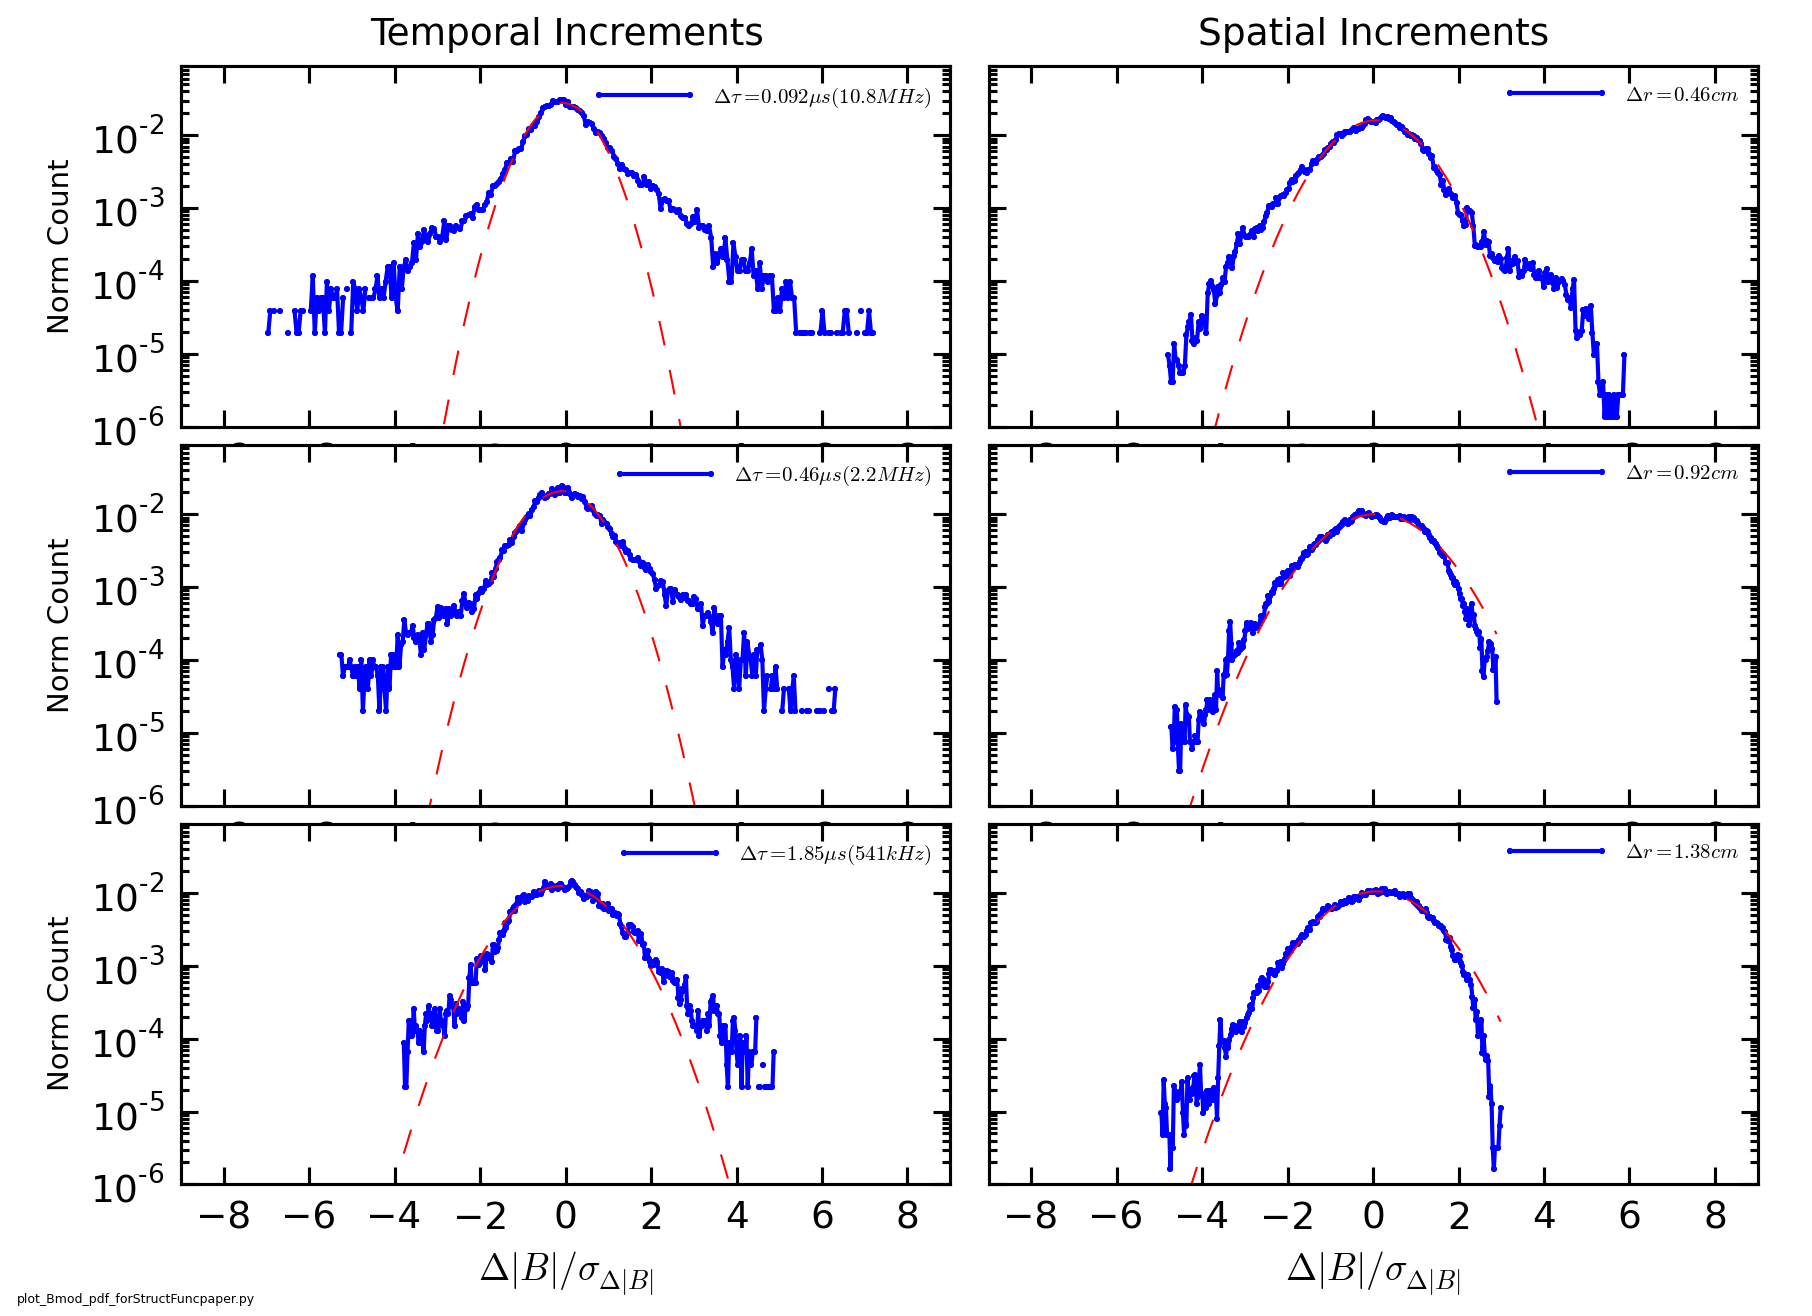
\includegraphics[width=17cm]{Bmod_pdf_temporal_and_spatial_100313Shots41to80_forStructFuncpaper.png}}
\caption{\label{fig:pdfs} }
\end{figure*}

Representative PDFs of both temporal and spatial magnetic field magnitude ($\Delta |B|$) increments are shown in Figure~\ref{fig:pdfs} with temporal PDFs on the left and spatial PDFs on the right. Each PDFs is scaled to its own standard deviation and total count so that they can be cross compared. The increments chosen for the temporal PDFs are $0.092\mu s$, $0.46\mu s$, and $1.85\mu s$ which correspond to frequencies of $10.8MHz$, $2.2MHz$, and $541kHz$ respectively. These three times also approximately correspond to three different regimes of the frequency spectra, called for lack of more accurate description the dissipation, transition and inertial region. All three PDFs exhibit intermittent behavior as indicated by the wings or ''fat tails`` for large fluctuation values which reflect larger counts compared to a true Gaussian distribution which is indicated by the dashed red curves. Note, though, that the qualitative ''level`` of intermittency decreases with increasing temporal increment, consistent with previous intermittency analyzes on SSX~\cite{schaffner2014a,schaffner2014b}, as well as solar wind results~\cite{bruno2013}.

The increments chosen for the spatial PDFs are $0.46cm$, $0.92cm$, and $1.38cm$, which corresponds to the minimum, double the minimum, and triple the minimum separation possible given the probe array in the SSX. Unlike the temporal data, the spatial data is not believed to probe any as far into dissipation range scales (for reference, an ion inertial length of 0.6cm  and an ion gyroradius of 0.1cm is calculated in this plasma). Thus the spatial data is likely representative of inertial range turbulence and at most transition range. The resulting PDFs support this notion as they tend to have a more Gaussian-like feature for small fluctuations and only slightly elevated tails. There does appear to be a trend toward increasing Gaussian-ness with increasing increment similar to the temporal data. The curves do no appear as smooth as the temporal data though, as the histograms have larger breaks---in particular, the $0.46cm$ increment PDF. This potentially reflects both a lower amount of increment statistics available for the spatial measurement as well as the possible variations in the PDF due to spatial variation. 

As discussed before, the use of PDFs of increments can clearly demonstrate the lack or presence of intermittent behavior in a signal, however in a primarily qualitative way. In order to demonstrate quantitative scaling behavior, and be able to extra more physical interpretations from the data, a structure function analysis is needed and is discussed in the next section.

\section{Structure Functions and Scaling with Order}\label{sec:structs}

To produce a more quantitative metric from the PDFs of increments, one can calculate moments of the histogram to any order $p$, and for each time or spatial delay $\Delta x$. This is equivalent to calculating the structure function for the magnetic field increments,
%
\begin{equation}
S^{p}(\Delta x) = \langle|B(x_{j}+\Delta x)-B(x_{j})|^{p}\rangle
\label{eq:structfunc}
\end{equation}
%
where $p$ is the order of the power and the angle brackets indicate summation over all $j$ elements of B. Integer values of $p$ correspond to the moments of the PDF ($p=2$ is the second moment, $p=3$ is the third moment, etc.) though given the form of Equation~\ref{eq:structfunc}, $p$ is not restricted to integer values in the structure function formalization.

\begin{figure*}[!htbp]
\centerline{
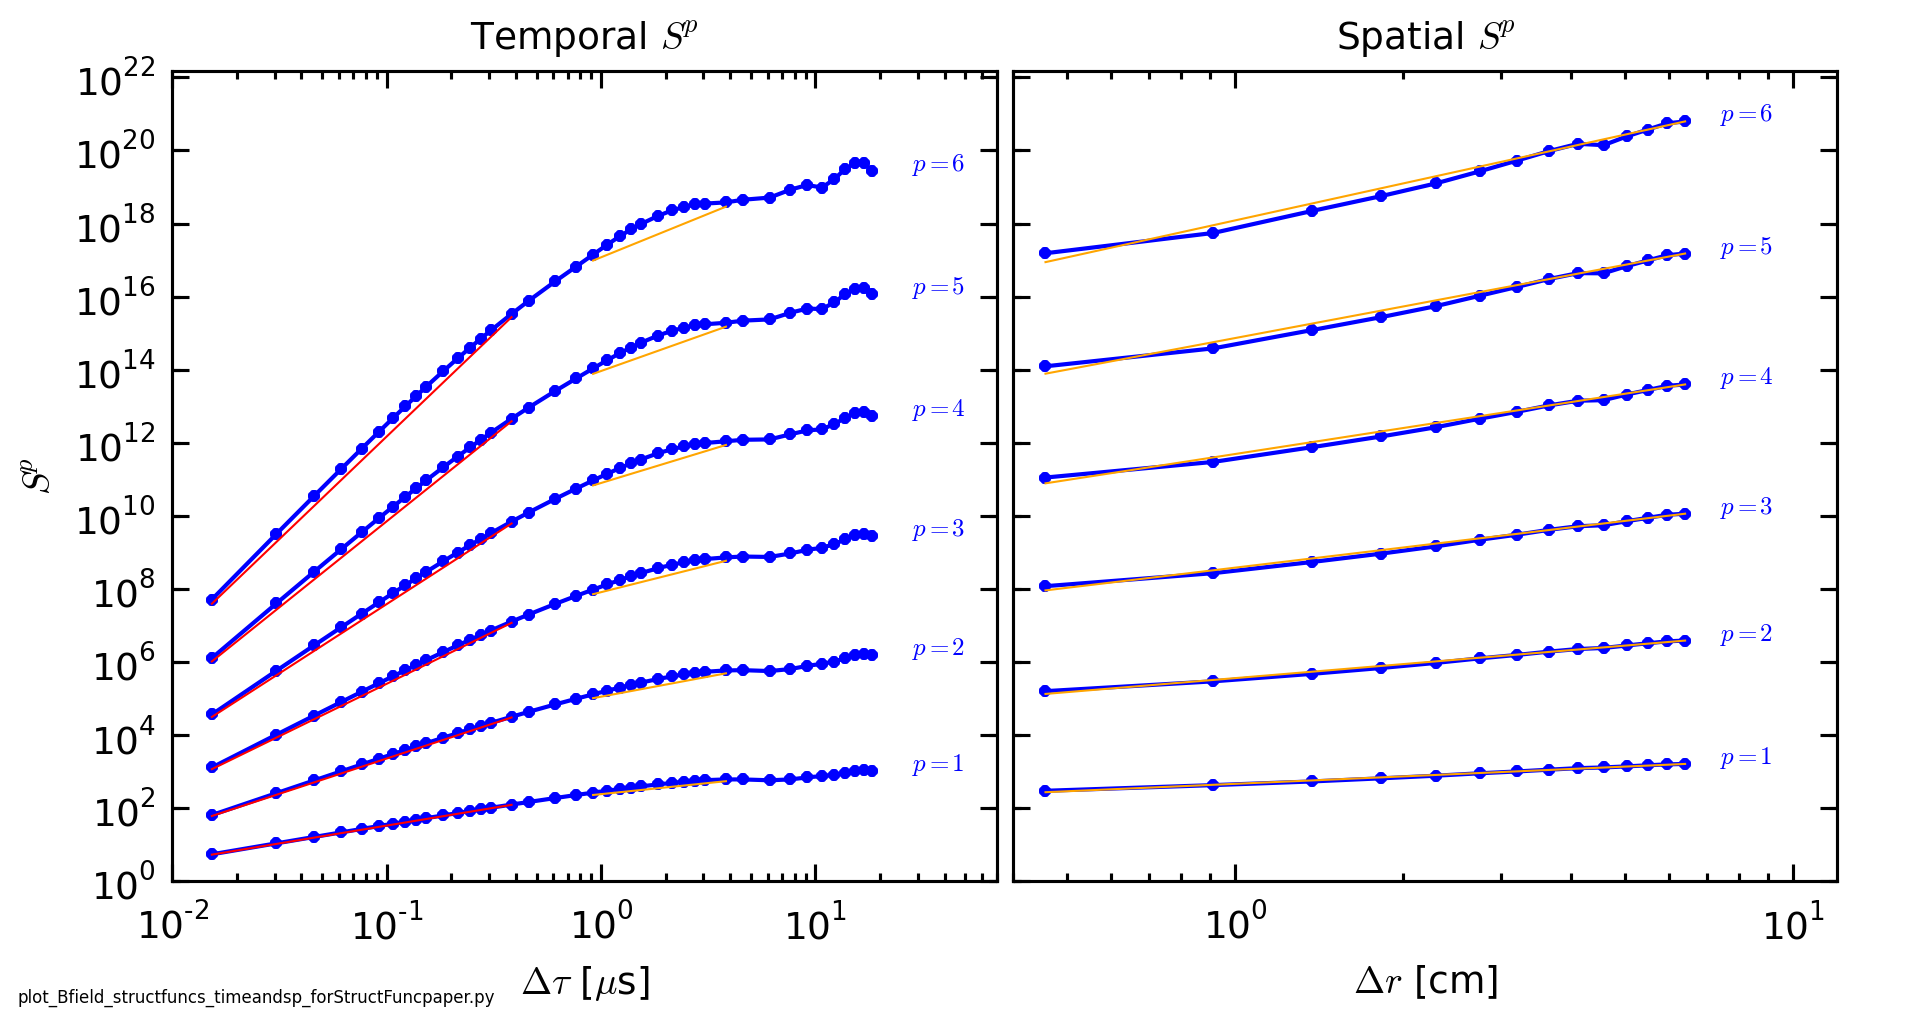
\includegraphics[width=17cm]{Bmod_timeandspace_StructureFunction100313Shots41to80_forStructFuncpaper.png}}
\caption{\label{fig:structfuncs} }
\end{figure*}

\begin{figure}[!htbp]
\centerline{
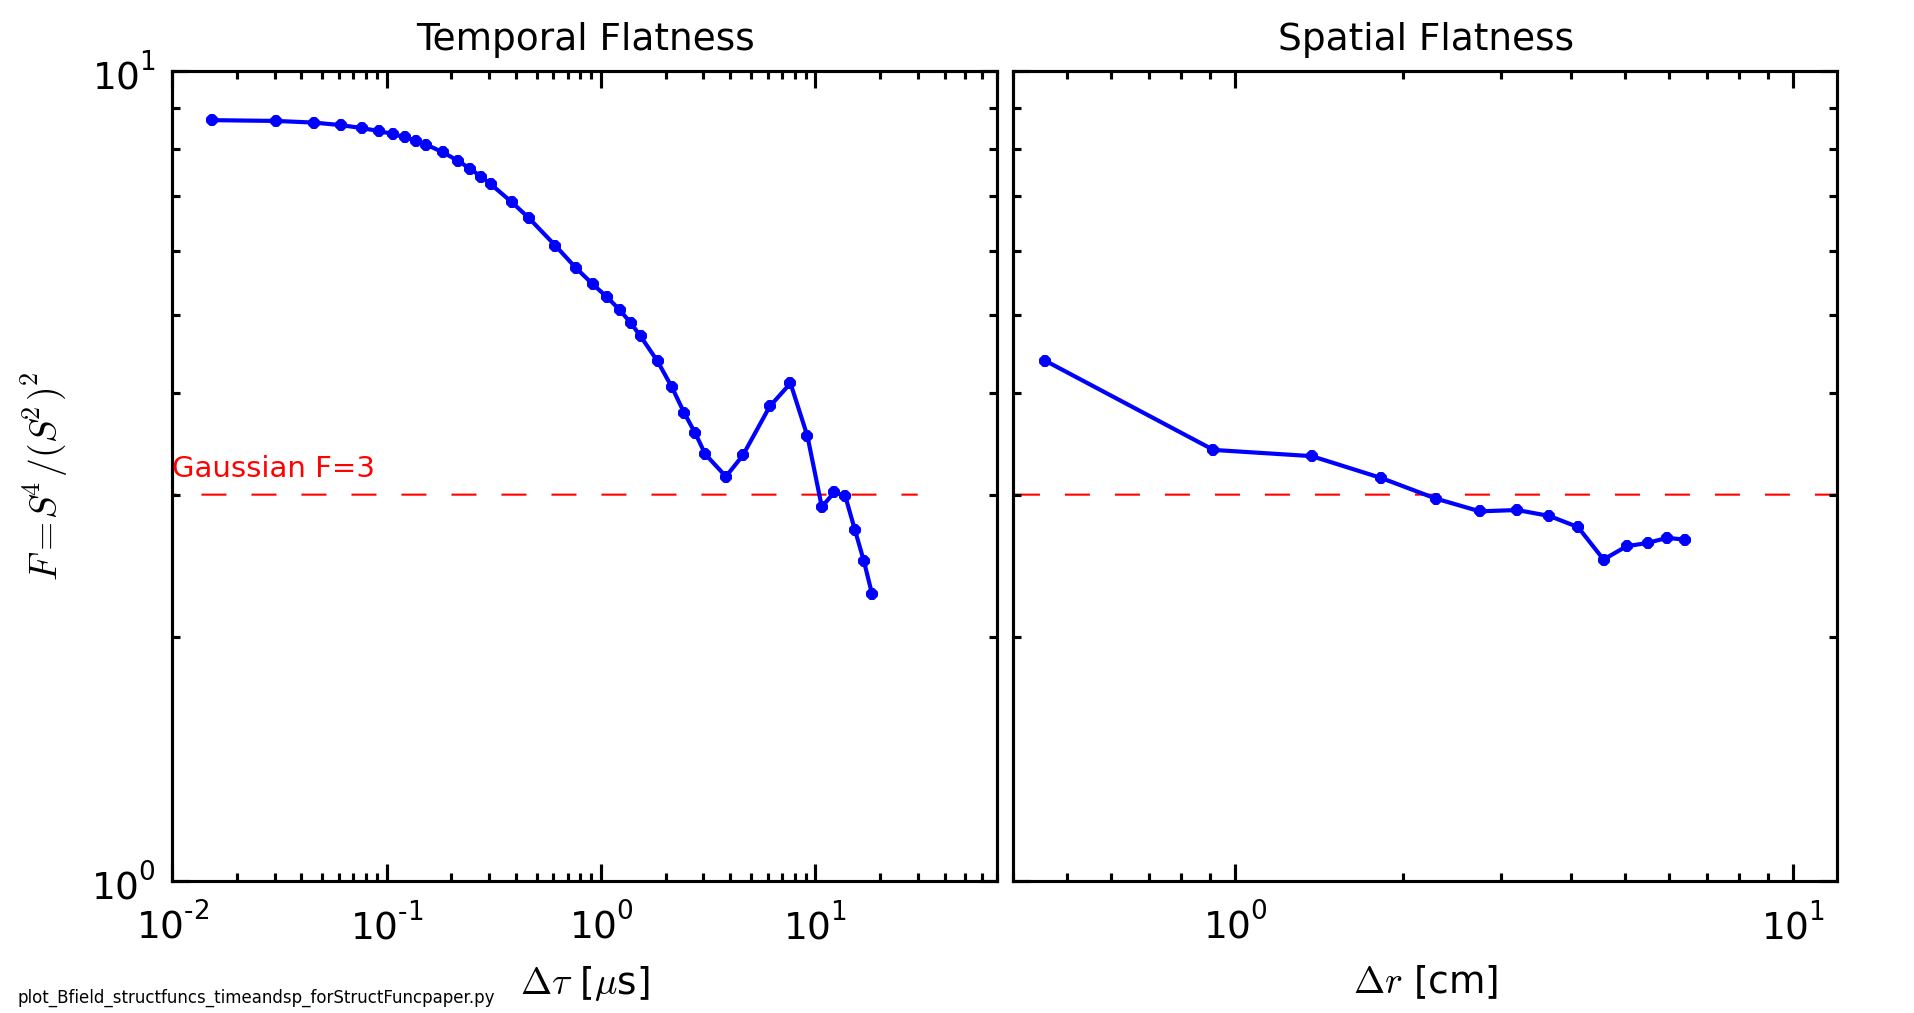
\includegraphics[width=8.5cm]{Bmod_timeandspace_Flatness100313Shots41to80_forStructFuncpaper.png}}
\caption{\label{fig:flatness} }
\end{figure}

Analysis of structure functions can provide a number of features of the fluctuations. The slope of the structure function indicates the relative level of intermittency compared between two signals. That is, the steeper the slope, the more intermittent (i.e. the larger the ''fat tails``) is the signal. A flat line is the extreme case and indicates a lack of intermittency in the signal. As one woud expect, the structure function of a timeseries generated from a normal distribution has a flat structure function. Changes in slope with scale indicates a change in intermittency as a function of scale. It should be noted that this trend is not a perfect predictor of the presense of intermitttency however. It can be shown that a time-series of fractional Brownian motion can be constructed with the same structure function slope(Hnat GRL 2003), but fBm produces a Gaussian probability distribution of increments (DOES IT?). However, when intermittency is known to be present based on the PDF of increments (as is true for this SSX dataset) then the relationship between slope and degree of intermittency generally holds true.

Figure~\ref{fig:structfuncs} shows the structure functions, $S^{p}(\Delta x)$, for temporal ($\Delta x = \Delta \tau$) data on the left and spatial ($\Delta x = \Delta r$) data on the right. The integer structure functions from $p=1$ to $p=6$ are shown. The structure functions vary as a function of $\tau$ or $r$ which confirms the presence of intermittency in the signal. For the temporal results, it is clear that this variation changes a function of time scale, with steeper slopes at small values of $\tau$ transitioning to shallower slopes at large values of $\tau$. This indicates that the relative degree of intermittency of the signal increases when analyzed at smaller scales. The transition range is also consistent with the transition from the inertial to the dissipation range of the cascade as determined by the change in spectral index of the frequency spectrum. This difference between inertial and dissipation range intermittency suggests that the physical mechanism underlying the dissipation dynamics has a more intermittent nature to it. Explanations for this behavior in the solar wind have typically center around the presence of current sheets in the magnetic turbulence(Osmin PRL 2014). The observation of this difference between dissipation and inertial range fluctuations in this laboratory plasma suggests a similar phenomena~\cite{schaffner2014b}. 

The spatial structure function do not show a variation with scale; however the slopes and thus the degree of intermittency is consistant with the temporal sturcture functions in the inertial range. Since the spatial meausrements can only probe inertial range scales in the plasma, this result supports the distinction between dissipation and inertial range intermittency seen in the temporal data.

A final characteristic, self-similarity of the turbulence, can be extracted from the structure function analysis by examining the slope of the structure functions as a function of order. In this context, the self-similarity is a qualitative measure of how alike fluctuations appear at different scales. A fractal from chaos theory is a construct that exhibits self-similarity. The red lines in Figure~\ref{fig:structfunc} are fits to the structure functions. In the temporal data, fits are done to two separate regions that correspond to the dissipation and inertial regions based on spectral frequency analysis, while the spatial data has only one fit for the entire region. A fit is made in each of these regions for each structure function using order $p$ which ranges between $0.1$ and $10$ in steps of $0.1$. The results of this scan are displayed in Figure~\ref{fig:slovesvsmom} for both time and space. The five separate magnetic field measurements are shown now, with inertial range fits indicate by solid lines and dissipation range fits indicate with dashed lines. In this construction, a timeseries that exhibits self-similarity would produce a line with a constant slope. As the increments are raised to increasingly higher powers, the value of the structure function should also increase exponentially. If the signal is self-similar, an increment between two points in the time series at one scale should have on average the same relative increment between two points at a different scale. In other words, a big fluctuation compared to a small fluctuation at one scale should appear to have the same relative ratio at a different scale. Thus, the structure function should change at a constant rate based on this ratio. If the signal is not self-similar, then the ratio is not constant and differences are increasingly accentuated by the raised exponent resulting in a non-linear scaling.

The original Kolmogorov turbulence theory in fact predicted a self-similar scaling such that the structure function slope would be equal to one-third of the power. The dashed purple line indicates this prediction in Figure~\ref{fig:slopesvsmom}. The inertial range curves for all five temporal magnetic measurements in Figure~\ref{fig:slopesvsmom}(a) sit relatively near the Kolmogorov theory line but none of the lines exhibiting completely linear behavior. This indicates that the inertial range fluctuations are not self-similar. The spatial curves in Figure~\ref{fig:slopesvsmom}(b) support this observation.

The dissipation range curves, in contrast, are clearly linear. This indicates that the dissipation range fluctuations are self-similar while also having a larger degree of self-similarity than inertial range fluctuations.

Like the Gaussian fits in Figure~\ref{pdfs}, the structure functions can be compared to the level of Gaussianness in the signal. Using a normalized structure function, a Gaussian timeseries would have a constant vale. For example, taking the normalized fourth order structure function (called kurtosis or flatness) yields a value of 3. 

%To see intermittency most clearly, need a normaloized structue function. unnormalized Strcture function demonstrates a distinctive change in the scaling at different time scsales. that is different scaling behavior as a function of tau. we can model the scaling as S = a*tau^\psi

\begin{figure}[!htbp]
\centerline{
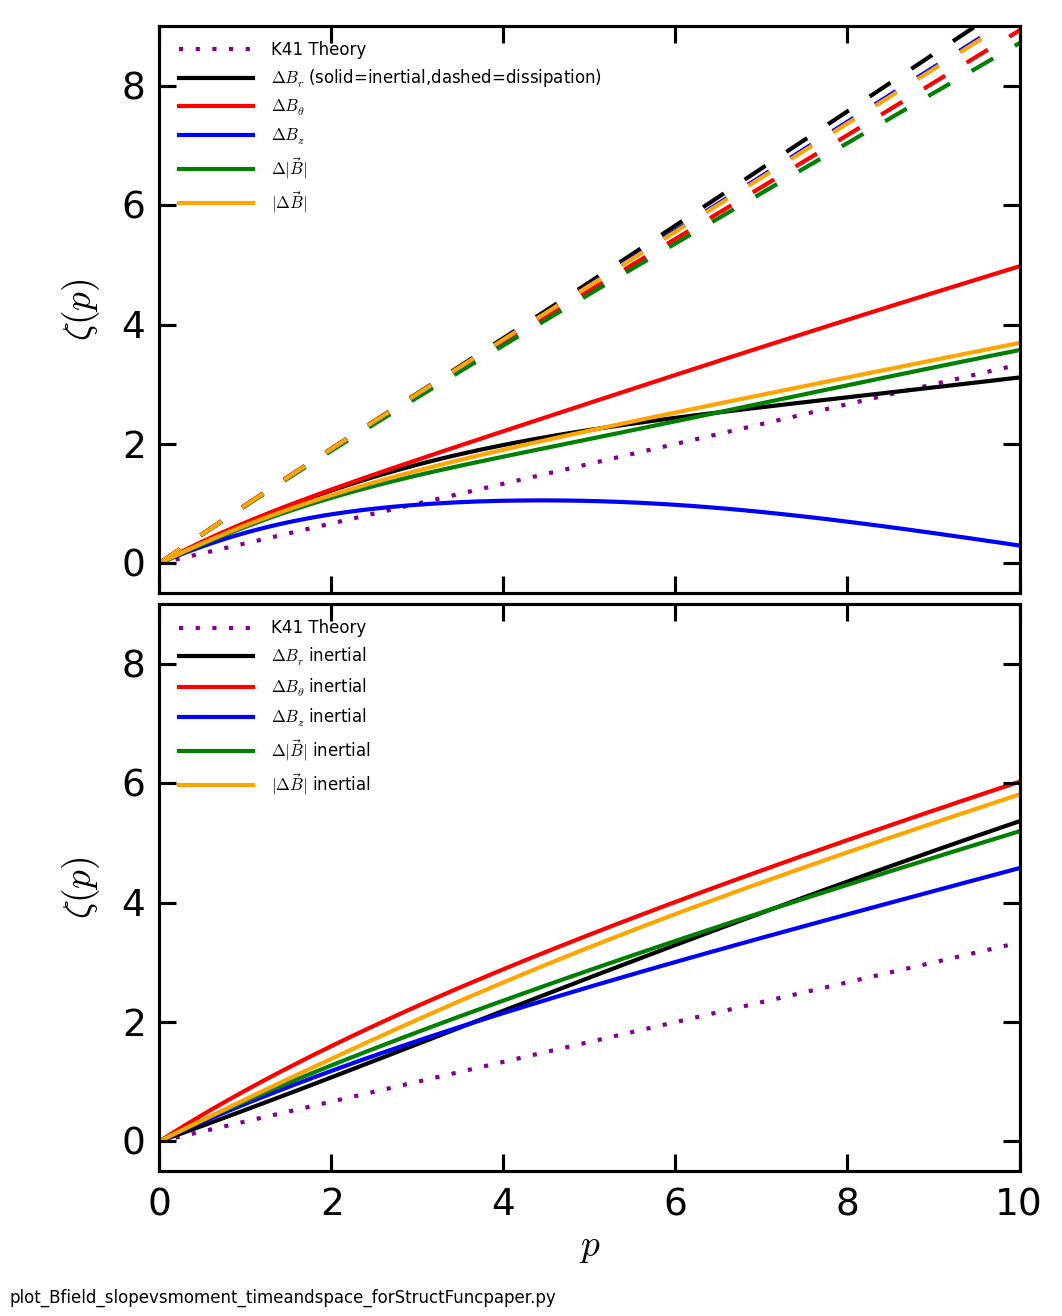
\includegraphics[width=8.5cm]{Bfield_StructureFunctionSlope_vs_Moment_timeandspace_100313Shots41to80_forStructFuncpaper.png}}
\caption{\label{fig:slopevsmom} }
\end{figure}

\section{Helicity Scaling}

The structure function analysis is also used to examine the effect of varying the amount of magnetic helicity in the plasma on the intermittency and self-similarity of the magnetic fluctuations. Previous work has shown that the degree of intermittency in fluctuations of $\dot{B}=dt/dB$ (not $B$), as determined by a calculation of the flatness, increases on averaged with an increasing amount of injected magnetic helicity~\cite{schaffner2014b}. This work revisits that result by examining the trend in $B$ using unnormalized structure functions and the resulting relationship between structure function slope and $p$. 

\begin{figure}[!htbp]
\centerline{
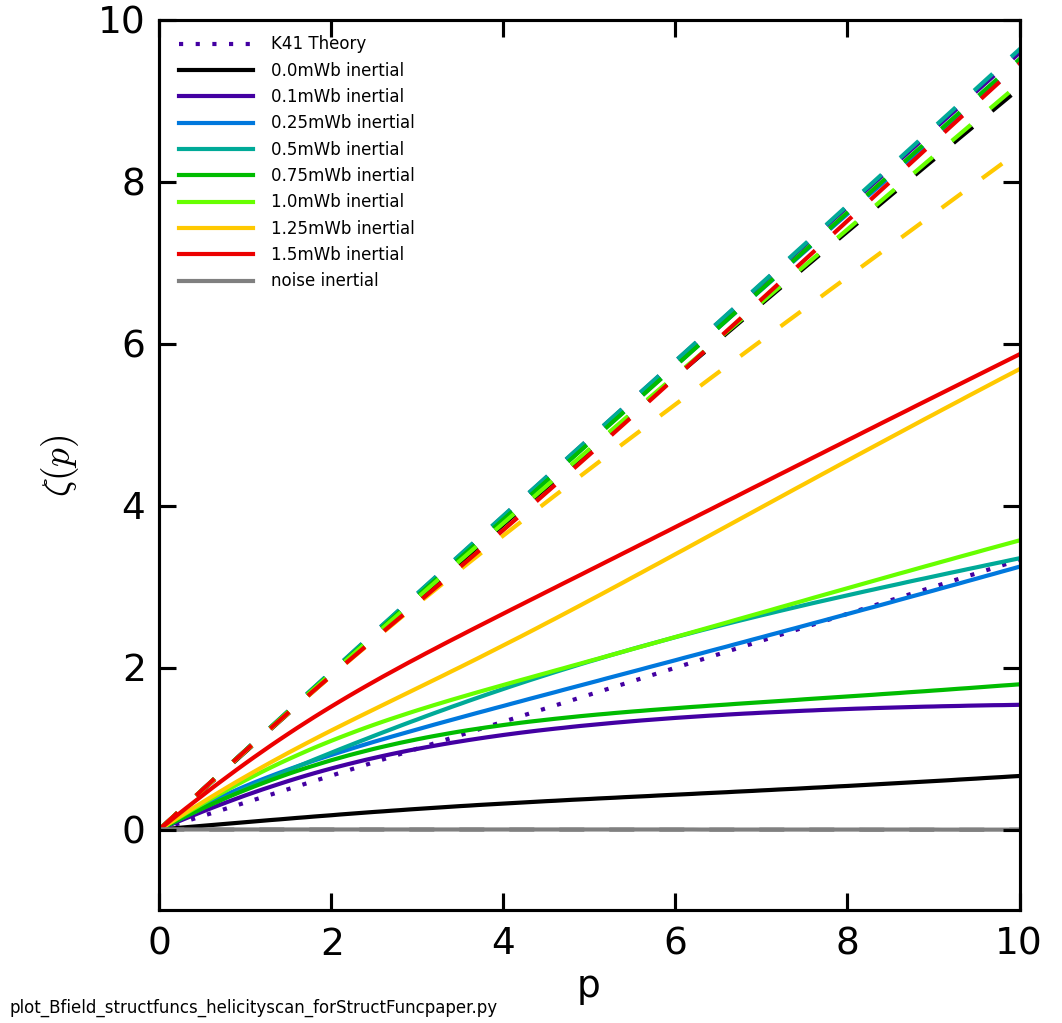
\includegraphics[width=8.5cm]{Bmod_StructureFunctionSlope_vs_Moment_helicityscan.png}}
\caption{\label{fig:helscan} }
\end{figure}

Figure~\ref{fig:helscan} shows the slope versus order for eight different helicity states for inertial range fluctutations (solid lines) and dissipation range fluctuations (dashed lines) Recalling that the steepness of the slope is indicative of relative degree of intermittency, the order of the inertial range curves for each helicity indicates increasing intermittency with increasing helicity, again consistent with the findings for an analysis of $\dot{B}$ timeseries~\cite{schaffner2014b}. However, the structure function analysis here further shows that with the exception of the zero helicity state, the inertial range turbulence for any helicity is not self-similar. The dissipation range lines, however, show that the dissipation range intermittency is self-similar regardless of the amount of injected magnetic helicity in the plasma.

\section{Discussion}

The value of this intermittency and structure function analysis lies in the ability to connect the observed trends to possible physical mechanisms. The most interesting result of this analysis is the observed distinction between inertial and dissipation range intermittency and self-similarity characteristics.

%physical connections

\section{Conclusions}\label{sec:conclusions}

% ----------------------------------------------------------------
\section*{Acknowledgements}
  We gratefully acknowledge many useful discussions with William Matthaeus, Greg Howes, Kris Klein, Robert Wicks, Jason TenBarge and Adrian Wan. This work has been funded by DOE OFES and NSF CMSO.  The simulations were performed using the advanced computing resources (Cray XC30 Edison system) at the National Energy Research Scientific Computing Center.
% ----------------------------------------------------------------
\section*{References}
\begin{thebibliography}{99}

\bibitem{bruno2013}
R. Bruno and V. Carbone. Living Rev Solar Phys {\bf 10} (2013).

\bibitem{alexandrova09} O. Alexandrova, J. Saur, C. Lacombe, A. Mangeney, J. Mitchell, S.J. Schwartz, and P. Robert. Universality of Solar Wind Turbulent Spectrum from MHD to Electron Scales. Phys. Rev. Lett. {\bf 103} 165003 (2009).

\bibitem{sahraoui09} F. Sahraoui, M.L. Goldstein, P. Robert and Yu. V. Khotyaintsev. Evidence of a Cascade and Dissipation of Solar-Wind Turbulence at the Electron Gyroscale. Phys. Rev. Lett. {\bf 102} 231102 (2009).

\bibitem{sahraoui06} F. Saharoui, G. Belmont, L. Rezeau, N. Cornilleau-Wehrlin, J.L. Pincon, A. Balogh. Anistropic Turbulent Spectra in the Terrestrial Magnetosheath as Seen by the Cluster Spacecraft. Phys. Rev. Lett. {\bf 96} 075002 (2006).

\bibitem{yordanova08} E. Yordanova, A. Vaivads, M. Andre, S.C. Buchert and Z. Voros. Magnetosheat Plasma Turbulence and Its Spatiotemporal Evolution as Observed by the Cluster Spacecraft. Phys. Rev. Lett. {\bf 100} 205003 (2008).

\bibitem{goldstein95} M.L. Goldstein, D.A. Roberts, and W.H. Matthaeus. Magnetohydrodynamic Turbulence in the Solar Wind. Annu. Rev. Astron. Astrophys. {\bf 33} 283-325 (1995).

\bibitem{tumarsch95} C.-Y. Tu and E. Marsch. MHD Structures, Waves and Turbulence in the Solar Wind: Observations and Theories. Space Sci. Rev. {\bf 73} 1-210 (1995).

\bibitem{podesta07} J.J. Podesta, D.A. Roberts, and M.L. Goldstein. Spectral Exponents of Kinetic and Magnetic Energy Spectra in Solar Wind Turbulence. ApJ. {\bf 664} 543-548 (2007).

\bibitem{chen13} C.H.K. Chen, S. Boldyrev, Q. Xia, and J.C. Perez. Nature of Subproton Scale Turbulence in the Solar Wind. Phys. Rev. Lett. {\bf 110} 225002 (2013).

\bibitem{montgomery81} D. Montgomery and L. Turner. Anistropic magnetohydrodynamic turbulence in a strong external magnetic field. Phys. Fluids {\bf 24} 825 (1981).

\bibitem{matthaeus90} W.H. Matthaeus, M.L. Goldstein, D.A. Roberts. Evidence for the Presence of Quasi-Two-Dimensional Nearly Incompressible Fluctuations in the Solar Wind. J. Geophys. Res. {\bf 95} 20673 (1990).

\bibitem{goldreich95} P. Goldreich and S. Sridhar. Toward a Theory of Interstellar Turbulence II. Strong Alvenic Turbulence. ApJ. {\bf 438} 763 (1995).

\bibitem{zhou04} Y. Zhou, W.H. Matthaeus and P. Dmitruk. Magnetohydrogynamic turbulence and time scales in astrophysical and space plasmas. Rev. Mod. Phys. {\bf 76} 1015 (2004).

\bibitem{boldyrev06} S. Boldyrev. Spectrum of Magnetohydrodynamic Turbulence. Phys. Rev. Lett. {\bf 96} 115002 (2006).

\bibitem{dasso05} S. Dasso, L.J. Milano, W.H. Matthaeus, and C.W. Smith. Anistropy in Fast and Slow Solar Wind Fluctuations. ApJ. {\bf 635} L181 (2005).

\bibitem{horbury08} T.S. Horbury, M. Forman, S. Oughton. Anisotropic Scaling of Magnetohydrodynamic Turbulence. Phys. Rev. Lett. {\bf 101} 175005 (2008).

\bibitem{podesta09} J.J. Podesta. Dependence of Solar-Wind Power Spectra on the Direction of the Local Mean Magnetic Field. ApJ. {\bf 698} 986 (2009).

\bibitem{perri09} S. Perri, E. Yordanova, V. Carbone, P. Veltri, L. Sorriso-Valvo, R. Bruno, and M. Andre. Magnetic turbulence in space plasmas: Scale-dependent effects of anisotropy. J. Geophys. Res. {\bf 114} A02102 (2009).

\bibitem{wicks10} R.T. Wicks, T.S. Horbury, C.H.K. Chen, A.A. Schekochihin. Power and spectral index anisotropy of the entire intertial range of turbulence in the fast solar wind. Mon. Not. R. Astron. Soc. {\bf 407} L31 (2010).

\bibitem{he11} J.-S. He, E. Marsch, C.-Y. Tu, Q.-G. Zong, S. Yao, and H. Tian. Two-dimensional correlation functions for density and magnetic field fluctuations in magnetosheath turbulence measured by the Cluster spacecraft. {\bf 116} A06207 (2011).

\bibitem{horbury12} T.S. Horbury, R.T. Wicks, C.H.K. Chen. Anisotropy in Space Plasma Turbulence: Solar Wind Observations. Space Sci Rev. {\bf 172} 325-342 (2012).

\bibitem{belcher71} J.W. Belcher and Leverett Davis, Jr. Large-Amplitude Alfven Waves in the Interplanetary Medium, 2. J. Geophys. Res. {\bf 76} 3534 (1971).

\bibitem{smith06} C.W. Smith, B.J. Vasquez and K. Hamilton. Interplanetary magnetic fluctuation anisotropy in the inertial range. J. Geophys. Res. {\bf 111} A09111 (2006).

\bibitem{coles89} W.A. Coles and J.K. Harmon. Propagation Observations of the Solar Wind Near the Sun. ApJ. {\bf 337} 1023 (1989).

\bibitem{harmon05} J.K. Harmon and W.A. Coles. Modeling radio scattering and scintillation observations of the inner solar wind using oblique Alfven/ion cyclotron waves. J. Geophys. Res. {\bf 110} A03101 (2005).

\bibitem{roberts10} D.A. Roberts. Evolution of the spectrum of solar wind velocity fluctuations from 0.3 to 5 AU. J. Geophys. Res. {\bf 115} A121001 (2010).

\bibitem{robinson71} D.C. Robinson and M.G. Rusbridge. Structure of Turbulence in the Zeta Plasma. Phys. of Fluids. {\bf 14} 2499 (1971).

\bibitem{liewer85} P.C. Liewer. Measurements of Microturbulence in Tokamaks and Comparisons with Theories of Turbulence and Anomalous Transport. Nuc. Fus. {\bf 25} 543 (1985).

\bibitem{tynan09} G.R. Tynan, A. Fujisawa, and G. McKee. A review of experimental drift turbululence studies. Plasma Phys. Cont. Fus. {\bf 51} 113001 (2009).

\bibitem{howes12a} G.G. Howes, D.J. Drake, K.D. Nielson, T.A. Carter, C.A. Kletzing and F. Skiff. Toward Astrophysical Turbulence in the Laboratory. Phys. Rev. Lett. {\bf 109} 255001 (2012).

\bibitem{ren11} Y. Ren, A.F. Almagri, G. Fiksel, S.C. Prager, J.S. Sarff and P.W. Terry. Experimental Observation of Anisotropic Magnetic Turbulence in a Reversed Field Pinch Plasma. Phys. Rev. Lett. {\bf 107} 195002 (2011).

\bibitem{deWit13} T. Dudok de Wit, O. Alexandrova, I. Furno, L. Sorriso-Valvo, G. Zimbardo, Methods for Characterising Microphysical Processes in Plasmas, Space Sci. Rev. {\bf 0038-6308}, p. 1-29 (2013).

\bibitem{schaffner14a} D.A. Schaffner {\it et al.} Turbulence analysis of an experimental flux rope plasma. {\bf 56} 064003 (2014).

\bibitem{schaffner14b} D.A. Schaffner {\it et al.} Observation of turbulent intermittency scaling with magnetic helicity in an MHD plasma wind-tunnel. Accepted by PRL April 2014.

\bibitem{sorrisovalvo99}Sorriso-Valvo, L. {\it et al.} Geophys. Res. Lett. {\bf 26}, 1801–1804 (1999).

\bibitem{kiyani13} K.H. Kiyani, S.C. Chapman, F. Sahraoui, B. Hnat, O. Fauvarque, and Yu.V. Khotyainsev. Enhanced Magnetic Compressibility and Isotropic Scale Invariance at Sub-Ion Larmor Scales in Solar Wind Turbulence. ApJ. {\bf 763} 10 (2013).

\bibitem{sahraoui10} F. Sahraoui, M.L. Goldstein, G. Belmont, P. Canu and L. Rezeau. Three Dimensional Anisotropic {\it k} Spectra of Turbulence at Subproton Scales in the Solar Wind. Phys. Rev. Lett. {\bf 105} 131101 (2010).

\bibitem{barnes86}C.W. Barnes, J.C. Fernandez, I. Henins, H.W. Hoida, T.R. Jarboe, S.O. Knox, G.J. Marklin, K.F. McKenna. Experimental determination of the conservation of magnetic helicity from the balance between source and spheromak. Phys. Fluids {\bf 29} 3415 (1986).

\bibitem{zhang11} X. Zhang, D. Dandurand, T. Gray, M.R. Brown, and V.S. Lukin, Calibrated Cylindrical Mach Probe in a Plasma Wind Tunnel, Rev. Sci. Instr. {\bf 82}, 033510 (2011).

\bibitem{bondeson81} A. Bondeson, G. Markon, Z.G. An, H.H. Chen, Y.C. Lee, and C.S. Liu. Tilting instibility of a cylindrical spheromak. Phys. Fluids. {\bf 24} 1682 (1981).

\bibitem{jarboe93}T.R. Jarboe. Review of Spheromak Research. Plasma Phys. Cont. Fus. {\bf 36} 945 (1994).

\bibitem{taylor86} J. B. Taylor, Rev. Mod. Phys. {\bf 58}, 741 (1986).

\bibitem{clauset09}A. Clauset, C. Rohilla Shalizi, M.E.J. Newman, Power-law distributions in empirical data, SIAM Rev. {\bf 51}, 661703 (2009).

\bibitem{sarkar14}A. Sarkar, A. Bhattacharjee and F. Ebrahimi. Plasma $\beta$ Scaling of Anisotropic Magnetic Field Fluctuations in the Solar Wind Flux Tube. ApJ. {\bf 783} 65 (2014).

\bibitem{tenbarge12} J.M. TenBarge, J.J. Podesta, K.G. Klein and G.G. Howes. Interpreting Magnetic Variance Anisotropy Measurements in the Solar Wind. ApJ. {\bf 753} 107 (2012).

\bibitem{hamilton08} K. Hamilton, C.W. Smith, B.J. Vasquez and R.J. Leamon. Anistropies and helicities in the solar wind intertial and dissipation ranges at 1 AU. J. Geophys. Res. {\bf 113} A01106 (2008).

\bibitem{matthaeus12}W.H. Matthaeus, S. Servidio, P. Dmitruk, V. Carbone, S. Oughton, M. Wan and K.T. Osman. Local Anisotropy, Higher Order Statistics and Turbulence Spectra. ApJ. {\bf 750}, 103 (2012).

\bibitem{torrence98}C. Torrence, G.P. Compo, A practical guide to wavelet analysis. Bull. Am. Meteorol. Soc. {\bf 79}, 6178 (1998).

\bibitem{klein12} K.G. Klein, G.G. Howes, J.M. TenBarge, S.D. Bale, C.H.K. Chen and C.S. Salem. Using Synthetic Spacecraft Data to Interpret Compressible Fluctuations in Solar Wind Turbulence. ApJ. {\bf 755} 159 (2012).

\bibitem{chen12} C.H.K. Chen, C.S. Salem, J.W. Bonnell, F.S. Mozer and S.D. Bale. Density Fluctuation Spectrum of Solar Wind Turbulence between Ion and Electron Scales. Phys. Rev. Lett. {\bf 109} 035001 (2012).

%\bibitem{Belmabrouk98} Belmabrouk, H., and M. Michard (1998), Taylor length scale measurement by laser Doppler velocimetry, Exp. Fluids, 25, 69Ð76.

%\bibitem{Matthaeus05} Matthaeus, W. H. and Dasso, S. and Weygand, J. M. and Milano, L. J. and Smith, C. W. and Kivelson, M. G., Phys. Rev. Lett. 95, 231101 (2005) Spatial Correlation of Solar-Wind Turbulence from Two-Point Measurements

%\bibitem{Weygand07} Weygand, J. M., Matthaeus, W. H., Dasso, S., Kivelson, M. G., and Walker, R. J. (2007), J. Geophys. Res., 112, A10201.

%\bibitem{Weygand09} Weygand, J. M., Matthaeus, W. H., Dasso, S., Kivelson, M. G., Kristler, L. M., and Mouikis, C. (2009), J. Geophys. Res., 114, A07213.

%\bibitem{Weygand10} Weygand, J. M., Matthaeus, W. H., El-Alaoui, M., Dasso, S., and Kivelson, M. G. (2010), J. Geophys. Res., textit115, A12250.

%\bibitem{Weygand11} Weygand, J. M., Matthaeus, W. H., Dasso, S., and Kivelson, M.G. (2011), J. Geophys. Res., 116, A08120.

%\bibitem{Matthaeus08} Matthaeus W. H., Weygand, J. M., Chuychai, P., Dasso, S., Smith, C. W., and Kivelson, M. (2008), Astrophys. J., 678, L141.

%\bibitem{frisch95}Frisch, U. 1995, {\it Turbulence} (Cambridge: Cambridge Univ. Press)

%\bibitem{sorrisovalvo99}Sorriso-Valvo, L. {\it et al.} Geophys. Res. Lett. {\bf 26}, 1801–1804 (1999).

%\bibitem{wan12}Wan, M. {\it et al.} ApJ. {\bf 744} 177 (2012).

%\bibitem{sorrisovalvo01}Sorriso-Valvo, L. {\it et al.} Planet. Space Sci. {\bf 49}, 1193–1200 (2001).

%\bibitem{marrelli05}Marrelli, L. {\it et al.} Phys. Plasmas. {\bf 12}, 030701 (2005).

%\bibitem{Greco08}A. Greco, P. Chuychai, W. H. Matthaeus, S. Servidio and P. Dmitruk, Intermittent MHD structures and classical discontinuities, Geophys. Res. Lett. {\bf 35}, L19111 (2008).

%\bibitem{Greco09}Greco, A., Matthaeus, W. H., Servidio, S., Chuychai, P., and Dmitruk, P.: Statistical Analysis of Discontinuities in Solar Wind ACE Data and Comparison with Intermittent MHD Turbulence, ApJ {\bf 691}, L111 (2009).

%\bibitem{Wan09}Wan, M., Oughton, S., Servidio, S., and Matthaeus, W. H.: Generation of non-Gaussian statistics and coherent structures in ideal magnetohydrodynamics, Phys. Plasmas {\bf 16}, 080703 (2009).

%\bibitem{Servidio11b}Servidio, S. {\it et al}, J. Geophys. Res. {\bf 116}, A09102 (2011).

%\bibitem{Gray13} T. Gray, M. R. Brown, and D. Dandurand. Phys. Rev. Lett. {\bf 110}, 085002 (2013). 



%\bibitem{Taylor86} J. B. Taylor, Rev. Mod. Phys. {\bf 58}, 741 (1986).

%\bibitem{Matthaeus80} W.H. Matthaeus and D. Montgomery, Ann. N.Y. Acad. Sci. {\bf 357}, 203 (1980).





%\bibitem{wan12}M. Wan, K. T. Osman, W. H. Matthaeus, and S. Oughton, Investigation of intermittency in magnetohydrodynamics and solar wind turbulence: scale-dependent kurtosis, ApJ {\bf 744}, 171 (2012).

%\bibitem{Gray10}T. Gray, V. S. Lukin, M. R. Brown, C. D. Cothran, Three-dimensional reconnection and relaxation of merging spheromak plasmas, Phys. Plasmas {\bf 17}, 102106 (2010).

%\bibitem{goldstein94}Goldstein, M.L., Roberts, D.A. and Fitch, C.A. Jour. Geo. Res. {\bf 99} 11519-11538 (1994).

%\bibitem{ji95}Ji, H., Prager, S.C. and Sarff, J.S. Phys. Rev. Lett. {\bf 74} 2945 (1995).

%\bibitem{telloni12}Telloini, D. {\it et al.}. ApJ. {\bf 751} 19 (2012).

%\bibitem{matthaeusVelli11}Matthaeus, W.H. and Velli, M. Space Sci. Rev. {\bf 160} 145-168 (2011).

%\bibitem{greco12}A. Greco {\it et al.} ApJ. {\bf 749} 105 (2012).

\end{thebibliography}

\end{document}

